Um Die Strahlungsintensität zu messen, steht die in Abbildung \ref{aufbau}
gezeigte Apparatur zur Verfügung. Diese besteht im Wesentlichen aus einem
Geiger-Müller-Zählroh der über einen Verstärker an ein elektronisches
Zählwerk angeschlossen ist.
\begin{figure}[H]
  \centering
  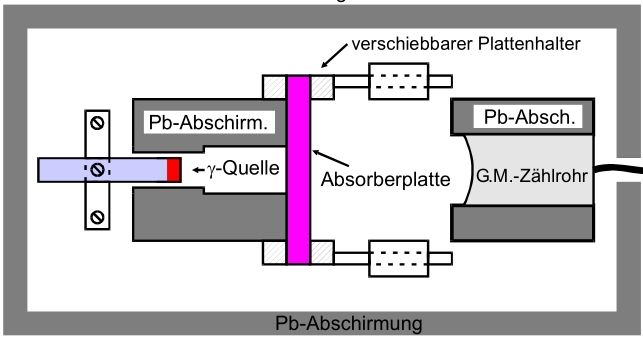
\includegraphics[width=8cm]{bilder/app.jpg}
  \caption{Schematischer Aufbau der Messvorrischtung \cite{704}.}
  \label{aufbau}
\end{figure}
\noindent
Durch einen Zeitgeber wird die Messzeit vorgegebe. Damit das Ergebnis nicht
übermäßig von äußeren Faktoren beeinflusst wird, ist die Apparatur zudem von einer
Blei-Wand umgeben.

\noindent
Zu Beginn der Messung wird eine Nullmessung durchgeführt, um den Nulleffekt zu
messen, welcher durch Sekundärprodukte von kosmischer Strahlung entsteht. Die
Nullmessung sollte mindestens $1100\sek$ betragen, da bei der $\beta$-Strahlung
nur geringe Zählraten auftreten.

\noindent
Nachdem der Nulleffekt bestimmt wurde, wird ein $\gamma$-Strahler ($^{137}\su{Cs}$
oder $^{60}\su{Co}$) in die Apparatur eingespannt. Nun werden verschiedene
Absorberplatten zwischen den Strahler und das Zählrohr gesetzt und die entsprechenden
$\gamma$-Absorptionskurven aufgenommen.
Anschließend wird die Messung mit einem $\beta$-Strahler ($^{99}\su{Tc}$) und einer
Aluminium-Absorberplatte wiederholt. Die aufgenommene Absorptionskurve wird dann
verwendet um die Maximalenergie des Strahlers zu bestimmen.
